\documentclass[aps,showpacs,twocolumn,floatfix,prx,superscriptaddress]{revtex4-1}
\usepackage{graphicx}
\usepackage{amsfonts}
\usepackage{amsmath}
\usepackage{amssymb}
\usepackage{upgreek}
\usepackage[usenames,dvipsnames]{color}

\begin{document}

\title{Dynamics of 1D polymer maps to ASEP}

\author{Wenwen Huang}
\author{Yen Ting Lin}
\author{Daniela Fr\"{o}mberg}
\author{Jaeoh Shin}
\author{Frank J\"{u}licher}
\author{Vasily Zaburdaev}
\affiliation{Max Planck Institute for the Physics of Complex Systems,
    N\"{o}thnitzer Str. 38, D-01187 Dresden, Germany}


\begin{abstract}
    Very often complex biological phenomena lead to a gold pot of statistical
    physics problems. In this article, we show how by reformulating the problem
    of chromosomal loop oscillations in the language of Brownian bridges we can
    unfold it into a set of related models from different fields of statistical
    physics and analytically solve them by essentially the same approach. We
    first demonstrate that a pinned polymer loop in the external force field can
    be approximated by a combination of Brownian bridge and Fermi-Dirac
    statistics, while the exact solution can be obtained via the Fermion integer
    partition problem. Next analogy we explore is to the asymmetric simple
    exclusion process with reflecting boundaries and thus solve for its
    statistics as well. Finally, in a way of demonstrating the results of such
    unexpected interplay of analogies, we show that the kinetic Monte-Carlo
    algorithm established for the exclusion process can be utilized to simulate
    the dynamics of the polymer loop and therefore stepping beyond equilibrium
    considerations. Thus we provide a unifying theoretical approach to a set of
    prototypical models of statistical physics which are of a broad interest to
    the fields of polymer physics, number theory, and single-file diffusion. 
\end{abstract}
\maketitle


\section{Introduction}
Through the decades of DNA research it has been demonstrated that simple polymer
models are extremely powerful tools to quantify various biological phenomena
involving dynamics and statistics of DNA molecules: from {\em in vivo}
mechanical properties of stretched DNA strands \cite{} to {\em in vitro}
chromosomal territories \cite{}, and hiC data \cite{}. Simple models, like the
freely jointed chain or random coil model \cite{}, often combine analytical
tractability and predictive power. Recently we have considered a problem of
chromosome alignment by the drag forces during meiosis in fission yeast \cite{}.
In polymer language this problem can be reformulated as finding the statistics
of a pinned polymer loop in the uniform external force field. By mapping the
original biological question to essentially a random walk problem we could solve
for statistics of chromosomes in quite complex three-dimensional geometry with
constraints. However, the developed theory only delivered predictions for the
equilibrium setting, while leaving the dynamics of the process beyond its reach.
%In a natural step towards understanding dynamics we decided first to consider
the simplest realization of the one-dimensional system that lead to a series of
interesting results.

In this paper, we show how the one-dimensional version of the pinned polymer
loop problem serves as a starting point of a chain of unexpected analogies that
interlink several fields of statistical physics. A synergy of the Brownian
bridge theory and Fermi-Dirac statistics serves as an asymptotic approximation
of the polymer loop statistics. However, exact solution can also be found by
solving the fermion number partition problem. We next notice that the dynamics
of the pinned polymer loop in an external force field can be mapped to an
asymmetric simple exclusion process (ASEP) with reflecting boundary conditions.
Via this link we can on the one hand immediately solve for the equilibrium
statistics of the ASEP model and on the other hand investigate the dynamics of
the polymer loop by means of the ASEP approach. To illustrate a possible
application of discovered similarities between very distinct models we show how
the ASEP model can be used to study the complex relaxation dynamics of polymers
in agreement with direct Brownian dynamics simulations of the original
three-dimensional system. Our results only cover the simplest geometries, but as
highlighted by the chromosome alignment problem, they can be naturally
generalized to include further additional constraints. The interrelation of
various prototypical statistical physics models, which we describe here, also
implies that methods developed for a particular problem can most probably be
ported to the other relative models as well. We thus think that the theoretical
results presented here will be of interest to an interdisciplinary scientific
community working in the fields of polymer physics, number theory, and
non-equilibrium statistical physics in general. 

The next Section II of the manuscript is devoted to the polymer loop model and
its equilibrium solution by a Brownian bridge theory and relation to the integer
number partition theory. We then turn to the dynamics and the ASEP framework in
Sec.III. In Sec.IV, We illustrate how the ASEP model can be utilized to study
the polymer relaxation dynamics. The last Section is reserved for the discussion
and conclusions.

\section{Statistics of the one-dimensional pinned polymer loop}
A polymer loop is a ubiquitous subject in polymer research pertinent to many
important biological phenomena \cite{}. For example, fission yeast uses the
viscous drag force to suppress fluctuations and align chromosomes for
recombination by pulling on chromosomes shaped in a loop \cite{}. For a constant
pulling speed this setting is equivalent to a pinned polymer loop in the uniform
external force field \cite{}. We start by setting up a one dimensional model of
this process.

We consider a classical freely jointed chain model consisting of $N+1$ beads
connected by $N$ rods; the rod length corresponds to the Kuhn length $a$ of the
polymer. The position of the $i^{\rm th}$ bead is denoted by $x_i$, $i\in\{0,1,
\ldots,N\}$. The looping condition suggests $x_0=x_N=0$. A constant external
force $F$ acts on every bead (except of pinned ones) and points in the positive
direction of the $x$-axis.  We define the orientation of the $i^{\rm th}$ rod as
$e_j:=(x_{j+1} - x_{j})/a$ and therefore $x_i = a\sum_{j=0}^{i} e_j$ where
$e_j=\pm 1$ and $i,j \in \left\{0, 1, \ldots, N-1\right\}$. In addition to
regular forces, there are random stochastic forces acting on the chain. We will
quantify their effect by an effective temperature $T$. We do not consider the
volume exclusion effects and bending energy in this model.

Note that in the absence of force this model is equivalent to a trajectory of a
one-dimensional unbiased random walk consisting of $N$ steps, where each step
corresponds to a monomer (rod) in the chain. This random walk, however, has to
start and end at the same point to fulfil the loop constraint. In mathematics,
it is known as the Brownian bridge problem and can be solved to find the
statistics of every bead position to be Gaussian with its variance depending on
the number of the bead \cite{}. Therefore we can outline the strategy of solving
the problem with a non-zero force: first find how the statistics of random walk
steps changes in the presence of force and then enforce the Brownian bridge
condition to form a loop. 

To find the statistics of random walk steps (rod orientations) we write down the
potential energy of the system:
\begin{equation}
    \label{eq:energy_polymer}
    E  = -\sum_{i=0}^{N-1} {Fx_i} = -Fa\sum_{i=0}^{N-1} \sum_{j=0}^{i}e_j, 
\end{equation}
%In addition, the looping condition gives
%\begin{equation}
%    \label{eq:looping}
%    \sum_{j=0}^{N-1} e_j = 0.
%\end{equation}
We now map the polymer model to a particle system. Note that the state of rod
orientation is binary, $e_j \in \left\{-1, +1\right\}$. We can map it to the
state of a lattice site which is either occupied by a particle, $Z_j = 1$, when
the rod points along the force or empty, $Z_j = 0$, if the rod points against
the force. The relation between $Z_j$ and $e_j$ is defined by a simple variable
transformation $Z_j := \left(e_j+1\right)/2$. The actual positions of polymer
beads are obtained by the back transformation
\begin{equation}
    \label{eq:z2x}
    x_i = a \sum_{j=0}^{i}{e_j} = a\left(2\sum_{j=0}^{i}{Z_j} -i\right).
\end{equation}
%Several examples of polymer configurations maps to particles on lattice sites are given
%in Fig. \ref{fig:schematic}. It is not difficult to see the boundary condition of
%lattice for the particle hopping model is reflecting boundaries. We will
%discuss more about this in section \ref{sec:asep}.
By exchanging the order of the double summation in Eq.
\eqref{eq:energy_polymer} and utilizing the loop condition  $\sum_{j=0}^{N-1}
e_j = 0$ we arrive at 
\begin{equation}
    \label{eq:energy_particle}
    E = \tilde{E} + \Delta E \sum_{j=0}^{N-1} j Z_j, 
\end{equation}
where $\tilde{E}= - N(N-1) \Delta E /2$ and $\Delta E = 2Fa$. The loop condition
implies a hard constraint of the total number of the particles $\sum_{j=0}^{N-1}
Z_j = N/2$ (there has to be equal number of steps along and against the force
field to return to the origin).

\subsection{Fermi-Dirac statistics of rod orientations}
In the energy expression \eqref{eq:energy_particle} one can immediately
recognize the energy of a system of $N/2$ Fermions distributed over $N$
equidistant energy levels $0, \Delta E, \ldots, (N-1) \Delta E$, where $Z_j$ can
be interpreted as an occupation number. Clearly the lowest energy of the system
corresponds to $Z_j = 1$ for $j < N/2$ and $Z_j=0$ otherwise (fully stretched
polymer loop). However, when the system is in contact with the thermal bath at
temperature $T>0$, it is possible to find other configurations. The equilibrium
Gibbs measure defines the probability of the system to be in a certain
configuration via the corresponding exponential Boltzmann factor.
%$\left\{Z_j\right\}_{j=0}^{N-1}$ is
%\begin{equation}
%    \label{eq:gibbs}
%    \mathbb{P}\left\{\left\{Z_j\right\}_{j=0}^{N-1}\right\} \propto \exp
%    \left[-\frac{\Delta E \sum_{j=0}^{N-1} j Z_j}{k_B T}\right]
%\end{equation}
%where $k_B$ is the Boltzmann constant. 
Interestingly, there are two possibilities to calculate those probabilities. 


The fixed total number or particles ($N/2$) corresponds to a picture of the
\emph{canonical ensemble} \cite{Chandler1987,Huang2001}: the system does not
exchange particles with its environment. However, the technical difficulty here
is in finding all degenerate microscopic states corresponding to the given total
energy of the system. Before venturing in this calculation we first look at the
alternative, approximate solution.

%While formally the equilibrium distribution is solved by
%\eqref{eq:gibbs}. But here the difficulty of obtaining the analytic solution due
%to the degeneracy of the system, i.e., some (total) energy levels contain
%multiple microscopic states. 

An alternative approach is to relax the fixed-number constraint, and use the
\emph{grand canonical ensemble}, which allows exchange of particles with an
external reservoir \cite{Chandler1987,Huang2001}, derive the probability
distribution of the microscopic states to construct a random walk model, and
then finally use the Brownian bridge condition to re-enforce the fixed-number
constraint \cite{Lin2015}. Under these assumptions, the statistics of the
particles is now given by a solution to the standard fermionic problem.  The
probability distribution of $Z_j$  is the {\em Fermi--Dirac} distribution:
\cite{Chandler1987,Lin2015}
\begin{subequations}
    \begin{align}
        \label{eq:discrete_prob}
        \mathbb{P} \left\{ Z_j = 1\right\} & =  \left\{1+\exp\left[\frac{ \Delta
                    E \left(j - \mu \right) }{k_B T}\right]\right\}^{-1}, \\
        \mathbb{P} \left\{ Z_j = 0\right\} & = 1 - \mathbb{P} \left\{ Z_j =
            1\right\},
    \end{align}
\end{subequations}
with a chemical potential $\mu = (N-1)/2$ obtained from the requirement that on
average there are $N/2$ particles in the system.  Noting the relation of $Z_j$
and the orientation of $j^{\rm th}$ rod $e_j = \left(2Z_j -1\right)$, the
probabilities \eqref{eq:discrete_prob} can be used to compute the distribution
of $e_j$. The Fermi--Dirac distribution shows that in the presence of the
external force field the first half of the steps is biased in the direction of
force, whereas the second half of steps has higher probability of pointing
against the force field.
%In this
%context, the famous Pauli exclusion principle---$Z_j$ can be either $0$ or
%$1$---corresponds to an almost trivial statement of each rod: either it points to
%the right ($Z_j=1$) or to the left ($Z_j=0$).  
We emphasize that only in the picture of the grand canonical ensemble, the
probability distributions of each rod orientation are mutually independent.%;
with a hard constraint of the particle number, $Z_j$'s
%are not independently distributed. In fact, the independence is the key for an
%analytic solutions of the equilibrium properties, such as \eqref{eq:gibbs}, are
%possible. 

Knowing the probability distribution of the occupation number (rod orientation),
their mean and variance can be easily calculated:
\begin{subequations}
    \begin{align}
        \label{eq:zmean}
        \mathbb{E}\left[Z_j\right] & =  \mathbb{P} \left\{ Z_j = 1\right\} ,\\
        \label{eq:zvar}
        \text{var}\left[Z_j\right] & = \mathbb{P} \left\{ Z_j = 1\right\} \cdot
        \left( 1 - \mathbb{P} \left\{ Z_j = 1\right\} \right) -
        \mathbb{E}\left[Z_j\right]^2.
    \end{align}
\end{subequations}
Now that we know the statistics of individual steps we can construct the
corresponding random walk process. Let us look at its trajectory connecting
beads $k$ and $l$, $l>k$ and the corresponding propagator $\rho(x_l=x|x_k=0)$.
Remarkably, according to the Lindeberg-Feller central limit theorem \cite{} this
propagator is  Gaussian with the mean and variance equal to the sum of mean and
variance of all individual steps leading from bead $k$ to $l$. We therefore
found the statistics of random walks governing the polymer loop in the presence
of the external force field. However, due to the grand canonical approach, such
random walks would return to the origin only on average. This random walk
properly reproduces the mean position of every bead, but it it is not enough to
estimate the fluctuations of its position. To work out the variance of the bead
position we have to enforce the loop condition.
 
%With \eqref{eq:zmean}, \eqref{eq:zvar}, a random walk is then built, satisfying
%the first and the second moments of the individual rods. Specifically, we
%construct a Gaussian random walk, which satisfies the conditional probability
%\begin{equation}
%    \label{eq:xmean}
%    \rho\left(x_{i+1} \vert x_i\right) =\exp\left\{ -\frac{\left[x_{i+1}- x_i -
%                a\mathbb{E}\left[Z_j\right]\right]^2}{4
%            \text{var}\left[Z_j\right]a^2}\right\}, 
%\end{equation}
%on a continuum domain $x \in \mathbb{R}$. 
\subsection{Imposing the Brownian bridge condition}
The Brownian bridge condition is a straightforward formulation of the condition
that a bead with an index $i$ is a part of the loop of length $N$. The bead $i$
belongs to the loop if two pieces of random walk trajectory of length $i$ and
$N-i$ respectively can meet at the position of the bead and belong to the same
loop. Thus the probability density function of finding the bead in a given
coordinate $x$ is given by
\begin{equation}
    \label{eq:bridge}
    \rho^L\left(x_i = x\right) = \frac{\rho\left(x_i = x \vert x_0 = 0\right)
        \rho\left(x_{N-i} = x \vert x_N = 0\right)}{\rho\left(x_N = 0 \vert x_0
            = 0\right)},
\end{equation}
where $ \rho\left(x_k = x \vert x_j = 0\right)$ are the propagators of the
corresponding random walk process. In case of the pinned polymer loop those
propagators are Gaussian distributions with a mean and variance obtained as a
sum of means and variances of all contributing individual steps of the random
walk. Importantly, because each propagator entering the above
Eq.(\ref{eq:bridge}) is Gaussian, the resulting $\rho^L\left(x_i = x\right)$ is
Gaussian as well. Its variance is given by
\begin{equation}
    \text{var}\left[x_i^L\right] =
    \frac{\sum_{j=0}^i\text{var}\left[Z_j\right]\sum_{j=N-i}^N\text{var}\left[Z_j\right]}{\sum_{j=0}^N\text{var}\left[Z_j\right]}
\end{equation}
We can now use these results and compare with direct Monte-Carlo simulations of
the one-dimensional pinned polymer loop in the external force field. In Fig. 1
we plot the mean (a) and variance (b) of every bead position for different
strengths of the external force field. With increasing force the polymer becomes
more stretched and fluctuations decrease. In the limit of zero force we recover
the well known result of the standard Brownian bridge problem. Although
calculating the sums involved in the estimation of the mean and variance does
not present any particular difficulty, for not too small temperatures the sums
can be approximated by integrals and evaluated explicitly (see Appendix A for
details). 

Therefore in this section we have shown that the combination of the Fermi--Dirac
statistics following from the grand canonical treatment of the system together
with the Brownian bridge condition for random walks allowed us to find an
excellent approximation for the statistics of the pinned polymer loop. In the
next section, for the sake of completeness we show how the same problem can be
addressed exactly in the canonical ensemble picture.

\subsection{Fermion integer number partition theory}
Although the above approach accurately estimates the mean and variance of
equilibrium position of $j^{\rm}$ bead, it is an approximated theory. Exact
analytic solution is possible in this particular model and helps to establishe
links to the number theory and theory of ASEP. First we change the basis of the
fermionic system from its microscopic configurations
$\left\{Z_0,Z_1,\ldots,Z_{N-1}\right\}$ to the total energy of the system.
Clearly, the energy can only take values $E_0, E_0+\Delta E, \ldots, E_0 + N^2
\Delta E / 4$ where $E_0$ is the ground state. In this picture, the probability
space is a one-dimensional lattice with finite support. Without loss of
generality, we set the constant energy $E_0=0$ and $\Delta E=1$. The difficulty
of this basis is to determine the degeneracy of the microscopic states which
have the same energy $E \in \left\{0,1,\ldots N^2/4\right\}$, sometimes referred
to as the ``density of the state'' in statistical mechanics
\cite{huang1987statistical} and condensed matter physics
\cite{sander2009advanced}. We denote the number of microscopic states with
energy $E$ to be $g(E)$; once $g(E)$ is known, the partition function of the
system can be formally derived in the canonical ensemble picture
\begin{equation}
\mathcal{Z}\left(T\right) = \sum_{E=0}^{N^2/4} g(E) \, \exp \left(-\frac{E}{k_B T}\right),
\label{eq:par_func}
\end{equation}
and consequently the equilibrium properties of the system can be derived from
it. 

Interestingly the problem of finding $g(E)$ can be solved with the help of the
closely related problem of integer partition in number theory
\cite{andrews1998theory}. The connection can be seen in the following way. We
label the micro-state of the system by how many energy units $E_i$ a fermion
with an index $i$ is excited from its ground state. The total energy of the
system is
\begin{subequations} \label{eq:partition}
\begin{align}
E= \sum_{i=1}^{N/2} E_i,
\end{align}
and by construction we have a constraint 
\begin{align}
N/2 \ge E_1 \ge E_2 \ge \ldots \ge E_{N/2} \ge 0. \label{eq:partition_constraint}
\end{align}
\end{subequations}
Equations \eqref{eq:partition} constitutes a restricted partition of the integer
$E$: $g(E)$ describes possible ways to partition an integer $E$ into $N/2$
non-increasing parts \cite{andrews1998theory}.

A very intuitive way to visualize the microscopic configurations is to use the
Young diagram \cite{andrews1998theory}, shown in the right panel of
Fig.~\ref{fig:schematic}. The black box in the row $i$ denotes the excited
energy $E_i$. With the constraint \eqref{eq:partition_constraint}, each row can
have at most $N/2$ black boxes, and the number of black boxes in $(i+1)^{\rm
    th}$ row cannot exceed the that in $i^{\rm th}$ row.  Then, $g(E)$ is the
number of possibilities to arrange $E$ black boxes onto the $N/2 \times N/2$
``checkerboard''. From the number theory \cite{andrews1998theory} the number of
ways to put $E$ black boxes onto an $K \times L$ checkerboard with
non-increasing number of black boxes per row, $\pi (K,L,E)$, can be calculated.
In our case $g(E)=\pi\left(N/2,N/2,E\right)$. Moreover we can find its
generating function:
%\begin{equation}
%\pi(K,L,E) = \pi(K,L-1,E) + \pi (K-1,L, E-L).
%\end{equation}
%which allows very efficient computations of the $g(E)=\pi\left(N/2,N/2,E\right)$. In addition, the generating function 
\begin{equation}
\Phi (q) := \sum_{E=0}^{N^2/4} g(E) q^E
\label{eq:generating}
\end{equation}
which turns out to be the Gaussian binomial coefficient
\begin{equation}
\Phi (q) = \left(\begin{array}{c} N \\ N/2 \end{array}\right)_q = \frac{\prod_{j=1}^{N} \left(1-q^j\right)}{\left[\prod_{j=1}^{N/2} \left(1-q^j\right)\right]^2}.
\label{eq:binomial}
\end{equation}
By comparing Eqs.(\ref{eq:par_func}) (\ref{eq:generating}) and
(\ref{eq:generating}) we can find an explicit and exact formula for the
partition function of the polymer loop problem:
\begin{equation}
\mathcal{Z}\left(T\right) = \frac{\prod_{j=N/2+1}^{N} \sum_{i=0}^{j}e^{-i\Delta E/k_{B}T}}{\prod_{j=1}^{N/2} \sum_{i=0}^{j}e^{-i\Delta E/k_{B}T}}.
\label{eq:par_func_exact}
\end{equation}

By knowing the exact partition function we can calculate the mean and variance
of each bead position. For larger $N$ the exact result is almost
indistinguishable from our approximate theory based on Brownian bridges
approach. However, for sufficiently small $N$ the difference becomes more
apparent (see Fig. X in Appendix B). Thus we have demonstrated that the polymer
loop model can be related and solved exactly in terms of the integer number
partitioning problem. This, however, is not the last analogy we are going to
utilize in this paper.

Here we have to note the connection of the considered problem to the ASEP setup
on an interval with reflecting boundaries \cite{}, where an analogous partition
function was calculated \cite{}. This demonstrates the equivalence of our model
of pinned polymer loop to the ASEP system with reflecting boundaries with
exactly one half of the lattice sites occupied by the particles. In the next
sections we further exploit this analogy to study the dynamics of the polymer
loop model.

\section{Asymmetric Simple Exclusion Process}\label{sec:asep}
Above we considered a one-dimensional lattice with $N$ lattice sites filled by
$N/2$ particles. So far we were concerned only with the equilibrium properties
of the system. However, by noticing the analogy to the ASEP model we can step
beyond equilibrium considerations and study the dynamics of our system. To
establish the link of the polymer loop model and the ASEP system we need to
understand the relation between polymer dynamics and hopping rules of the ASEP.
A particle occupying a lattice cite corresponds to a monomer of the polymer loop
pointing along the direction of force. Hopping of a particle on a lattice
corresponds to the flipping of two monomers connecting to the same bead and
having the opposite orientations with respect to the force field (see
illustration in Fig. 3). During this flip, the bead has to travel a distance of
$\pm2a$. Indeed, just like in the exclusion process, the flip can occur only if
there is a ``free'' lattice site. The asymmetry of the flipping results from the
force acting on the beads: if as a result of the flip the bead will move along
the force, it will be energetically more favourable move than flipping the bead
against the force. We can now formalize such dynamics by using the language of
the ASEP model \cite{Derrida1998,Schutz2001}. 
 
 We denote the rate of particle hopping to right and left with $\alpha$ and
 $\beta$ respectively. From the detailed balance relation we have 
\begin{equation}
    \alpha P_{n} = \beta P_{n+1} \label{eq:db}
\end{equation}
where $P_{n}$ is the probability of a particle sitting on the $n^{\rm{th}}$
site. The ratio of rates (and thus of the neighboring occupation probabilities)
is proportional to the Boltzmann factor with the energy difference between the
two states:
\begin{equation}
    \beta / \alpha = P_{n} / P_{n+1} = \exp{(-\Delta E / k_B T)},  \label{eq:r_divide_l}
\end{equation}
where  $\Delta E = 2Fa$.
The total hopping rate of a particle is determined by the temperature:
\begin{equation}
    \alpha + \beta = r_{\text{total}} \label{eq:l_plus_r}
\end{equation}
where $r_{\text{total}}$ is a quantity determined by the system's temperature.
Hopping of a particle to the neighboring lattice site corresponds to flipping of
two monomers and the displacement of the bead by a distance of $2a$. In the
force-free case this flipping happens due to random forces acting on the bead.
Note that in the strictly one-dimensional setting, the monomers can not
continuously turn, there are just initial and final states along or against the
field. However, to quantify the time required for making a flip we can relax
this limitation and imagine the bead continuously diffusing in space before it
manages to travel a distance of $2a$. The diffusion constant of the bead is
given by Einstein relation $D=k_{B}T/\gamma$, where $\gamma$ is the Stokes
friction $\gamma=6\pi R\eta$, $\eta$ is viscosity of the surrounding fluid, and
$R$ is the radius of the bead. We can now use this relation to estimate the time
constant and therefore the total hopping rate:
\begin{equation}
D=\frac{4a^2}{2\tau_0}=\frac{k_{B}T}{\gamma}; \quad \tau_0=\frac{2\gamma a^2}{k_{B}T}=r_{\text{total}}^{-1}.
\end{equation}
Finally we obtain for the left and right hopping rates:
% With eq. \eqref{eq:l_plus_r} and eq. \eqref{eq:r_divide_l}
%we can in principle solve $\alpha$ and $\beta$ uniquely. The key quantity here is
%$\Delta E$, which actually connects polymer and particle model. One can learn
%from the polymer and particle equivalence that one particle hopping the right
%corresponds to the change of two consecutive rods orientation from right-left to
%left-right. Thus the energy difference of the two configuration writes
%\begin{equation}
%    \Delta E = 2Fa
%\end{equation}
\begin{subequations}
    \label{eq:l_and_r}
    \begin{equation}
        \alpha  =  \frac{r_{\text{total}}}{1+\exp{(-2Fa / k_B T)}}
    \end{equation}
    \begin{equation}
        \beta  =   \frac{r_{\text{total}}\exp{(-2Fa / k_B T)}}{1+\exp{(-2Fa / k_B
                T)}} \\
    \end{equation}
\end{subequations}
Hopping rates determine the dynamics of the polymer (particle) configurations,
but we also need to specify the boundary conditions and if there any additional
constraints on the number of particles. The pinned polymer loop corresponds to
exactly $N/2$ particles hopping on $N$ lattice sites and therefore to reflecting
boundary conditions. The mapping can be generalized to other cases, for example
an un-pinned polymer loop corresponds to $N/2$ particles on $N$ lattice sites
with periodic boundaries, free polymer chain corresponds to an open lattice of
length $N$ filled by arbitrary (but not larger than $N$) number of particles. 

ASEP is one of the fundamental models of non-equilibrium statistical physics
with a wealth of important analytical results. However, not so many works are
dealing with the particular case of reflective boundary conditions. One
important contribution is due to Schuetz \cite{} where the partition function
identical (Check!) to Eq.(\ref{eq:par_func_exact}) was derived. Here our main
motivation is to get an insight on the dynamics of the polymer loop. We therefore
make use of the described analogy between the polymer problem and ASEP and
employ highly efficient kinetic Monte-Carlo simulations ubiquitous for particle
systems. 

\section{Relaxation dynamics}

% With the ASEP analogy of polymer dynamics, we are ready to go deeper to analyze
% the non-equilibrium properties of the polymer system. One of the typical
% quantities people interested about dynamics is relaxation time, denote by
% $\tau$ here. The protocol here is as following, firstly the trajectories of
% particle on ASEP is recorded and then transformed to bead position of polymer
% by eq.  \eqref{eq:z2x}, finally relaxation time is fitted from auto-correlation
% function (ACF) of interested observables such as gyration radius defined
% by $\mathbf{R}_g^2:= \frac{1}{N}\sum_{i=1}^N{\left(\mathbf{r}_i -
%         \mathbf{r}_{CM}\right)^2}$.
%
% To get trajectories of hopping particle, we employ the Kinetic Monte Carlo
% simulation\cite{Gillespie1976}, which is very fast and efficient compare to
% Molecular Dynamics simulation of polymer. By transform to the picture of
% polymer, we obtain the dynamical behavior illustrate in Fig.
% \ref{fig:transient}. 
%
% ACF of gyration radius is calculated based on the information of beads position.
% As we see the ACF($Rg$) decays exponentially with time
% lag. However, we also observe a effect of multiple relaxation modes indicated
% by the beginning part of the curve, especially in the case of strong external
% force. This multi-mode behavior is predicted in Rouse model. 
% Practically, relaxation time is fitted in the decaying regime where the slope
% is most flat, which corresponds to the longest relaxation mode.   
% \begin{figure}[htpb]
%     \centering
%     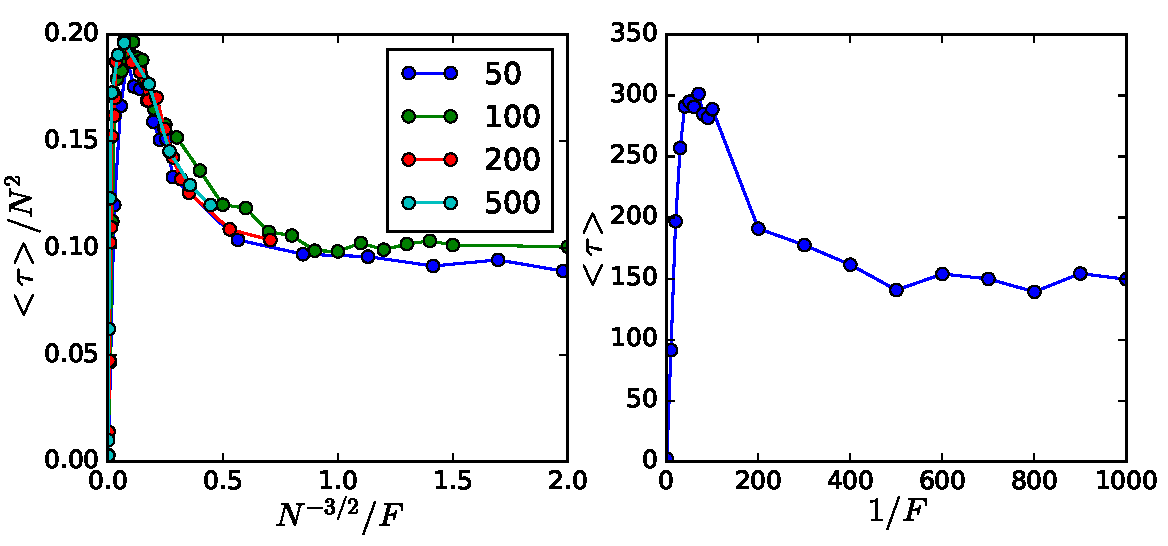
\includegraphics[width=1.0\linewidth]{tauscaling}
%     \caption{Relaxation time of gyration radius varies with external force. Left
%         1D, right 3D.}
%     \label{fig:tauscaling}
% \end{figure}
% We interested in how the relaxation time varies with the external force field.
% So we fixed the temperature $T$ and total hopping rate $r_{total}$ in our model and
% simulate the relaxation behavior for different external force. One would
% intuitively expect a monotonic decreasing as $F$ grows. Interestingly, we found a
% non-monotonic behavior contrast to the expectation, i.e. there is peak which
% marks a slowest relaxation time in a weak external force regime. See in Fig.
% \ref{fig:relaxation}. To verify the non-monotonic behavior is not artificially
% introduced by the reduction of the model, we perform a 3D Brownian dynamics
% simulation of pinned bead-rod loop with the same settings. We successfully
% reproduced the same behavior of relaxation time varies with external force ---
% non-monotonic, as illustrate in Fig. \ref{fig:relaxation}. Moreover,
% experimental evidence of this non-monotonic relaxation behavior is also
% reported with a similar setting in \cite{Doyle2000}.
%
% A simple theory of relaxation time can be obtained by Rouse
% model\cite{Rouse1953,Doi1986}.
% However, the rouse model cannot explain the non-monotonic behavior for
% relaxation time and external force. In fact, classical Rouse theory predicts the
% relaxation time is irrelevant with the external force. The main reason for break
% down of Rouse theory is due to the non-extensible rigid rod in our model, in
% contrast to the unrealistic infinitely extensible spring in Rouse model. On the
% other hand, Rouse theory correctly predicts the scaling law for relaxation time
% with system size when external force is not too strong, i.e. $\tau \propto N^2$
% when $1/F \gg 1$.
%
% The non-monotonic behavior can be better understood in the corresponding
% particle hopping picture. In the strong force case, all particles sit on the
% left half of the lattice sites. Only the right-most particle is free to hop
% right. In fact, because of the strong hopping bias to the left, even this
% particle is not easy to move. Thus a faster relaxation behavior is observed
% caused by the strong constraint. On the other hand, when there is totally no
% external force applied on the polymer beads, which means there is no bias for
% the particle hopping. In this case, the particle will finally evenly
% distributed on the lattices sites. The freedom of particle to move is confined
% by its neighbors, which is only $2$ lattice sites in average. Since the total
% hopping rate is fixed, the relaxation time is proportional to the accessible
% distance. In comparison, in the moderate force regime, particle distributed
% denser on the left part of lattice and sparser on the right part. The freedom
% for those particles on the right side to move is larger than the case of no
% external force, and the constraint is not so strong that these particles can
% still easily move around. These conditions lead to a longer relaxation time than
% the case with no force. 
%
% We now come back to discuss more about the scaling law of relaxation time with
% system size. As mentioned above, for relaxation time scales with $N^2$ when
% external force is not too strong, predicted by Rouse theory. But how about when
% the force is strong? It turns out relaxation time is irrelevant with system size
% in this case, i.e. $\tau \propto N^0$. We can again understand this easily
% in the particle hopping picture. When the external force is strong, the bias of
% particle hopping rate is thus strong. As a result, particles accumulate in the
% left side and only few right most particle can move. And the number of movable
% particle doesn't depend on the actual total number of particles (polymer size).
% In other words, in the case of strong force, only the tail part of the polymer is
% fluctuating, the size of this fluctuating blob is not related with the contour
% length of the polymer but increase as the external force decrease. Quantitative
% results are possible with this understanding and will be discussed in our
% future work. Another interesting scaling is how the peak position scales with
% the system size. We observe here a scaling of $N^{3/2}$, but lack of physical
% understanding of that.
%
\section{Conclusions}
In conclusion, we demonstrate that 1D polymer can be exactly mapped to a
particle hopping on lattice sites, i.e. ASEP.  We discussed the case of pinned
polymer loop in detail, shown the analytical equilibrium statistics drawing
from the mapping. Furthermore, the dynamics of polymer is also illustrated
in the mapped particle hopping picture. Interestingly, we found that even in
this simple model, there are a lot of non-trivial features such as relaxation
time varies with external force non-monotonically, and different scaling
behavior for relaxation time for different external force. An quantitative
explanation is given by picture of particles hopping on the lattices sites.  

The mapping from polymer to particle is not restricted in the case of pinned
polymer loop. Other generalizations can be investigated with the same mapping,
which leads to ASEP model with different boundaries and particle numbers. We
emphasize the generality of this mapping which can be applied to a huge class of
polymer problems. Moreover, the polymer dynamics beyond 1D is also possible to
model by multi-species ASEP model. There are still a lot of fascinating open
questions to discover in the future.

\begin{acknowledgments}
We would like to acknowledge stimulating discussions with M. Majumdar.\end{acknowledgments}

%\bibliography{oscillations}

\begin{thebibliography}{10}


\bibitem{alberts2002}
B.~Alberts,
  A.~Johnson,
  J.~Lewis,
  M.~Raff,
  K.~Roberts, and
  P.~Walter,
  \emph{Molecular Biology of the Cell, Fourth Edition}
  (Garland Science, New York, 2002),
  4th ed.

\bibitem{gerton2005}
J.~L. Gerton and
  R.~S. Hawley,
  Nat. Rev. Genet. \textbf{6},
  477 (2005).

\bibitem{villeneuve2001}
A.~M. Villeneuve
  and K.~J.
  Hillers, Cell
  \textbf{106}, 647 (2001).

\bibitem{McKee2004}
B.~D. McKee,
  BBA-Gene. Struct. Expr. \textbf{1677}, 165 
  (2004).

\bibitem{Egel2004}
R.~Egel,
  \emph{The Molecular Biology of Schizosaccharomyces pombe:
  Genetics, Genomics and Beyond}(Springer, Berlin-Heidelberg,
  2004).

\bibitem{davis2001}
L.~Davis and
  G.~R. Smith,
  Proc. Natl. Acad. Sci. U. S. A.
  \textbf{98}, 8395 (2001).

\bibitem{munz1994}
P.~Munz,
  Genetics \textbf{137},
  701 (1994).

\bibitem{wells2006}
J.~L. Wells,
  D.~W. Pryce, and
  R.~J. McFarlane,
  Yeast \textbf{23}, 977
  (2006).
  
 \bibitem{SM} See Supplemental Material at ... for detailed description of experimental procedures, numerical simulations, and the discussion of 3D fluctuations of the polymer loop.

\bibitem{ding1998oscillatory}
D.-Q. Ding,
  Y.~Chikashige,
  T.~Haraguchi,
  and Y.~Hiraoka,
  J. Cell Sci. \textbf{111},
  701 (1998).

\bibitem{vogel2009self}
S.~K. Vogel,
  N.~Pavin,
  N.~Maghelli,
  F.~J\"ulicher,
  and I.~M.
  Toli\'c-N\o rrelykke, PLoS Biol.
  \textbf{7}, e1000087
  (2009).

\bibitem{yamamoto2001dynamic}
A.~Yamamoto,
  C.~Tsutsumi,
  H.~Kojima,
  K.~Oiwa, and
  Y.~Hiraoka,
  Mol. Biol. Cell \textbf{12},
  3933 (2001).

\bibitem{yamamoto1999cytoplasmic}
A.~Yamamoto,
  R.~R. West,
  J.~R. McIntosh,
  and Y.~Hiraoka,
  J. Cell Biol.
  \textbf{145}, 1233 (1999).

\bibitem{ananthanarayanan2013dynein}
V.~Ananthanarayanan,
  M.~Schattat,
  S.~K. Vogel,
  A.~Krull,
  N.~Pavin, and
  I.~M. Toli\'c-N\o rrelykke,
  Cell \textbf{153}, 1526
  (2013).

\bibitem{koszul2009dynamic}
R.~Koszul and
  N.~Kleckner,
  Trends Cell Biol. \textbf{19},
  716 (2009).

\bibitem{ding2004dynamics}
D.-Q. Ding,
  A.~Yamamoto,
  T.~Haraguchi,
  and Y.~Hiraoka,
  Dev. Cell \textbf{6},
  329 (2004).

\bibitem{wynne2012dynein}
D.~J. Wynne,
  O.~Rog,
  P.~M. Carlton,
  and A.~F.
  Dernburg, J. Cell Biol.
  \textbf{196}, 47 (2012).

\bibitem{Doi1986}
M.~Doi and
  S.~Edwards,
  \emph{The theory of polymer dynamics, International series
  of monographs on physics} (Clarendon Press, Oxford,
  1986).
  
\bibitem{foot0}
{\color{blue} Since the recombination machinery, locally altering the properties of the chromatin, becomes active only after the homologous chromosomes come to close proximity, we assume the effective temperature to be spatially uniform.}

\bibitem{Revuz1999}
D.~Revuz and
  M.~Yor,
  \emph{Continuous Martingales and Brownian Motion,
  Grundlehren der mathematischen Wissenschaften} (Springer, Berlin-Heidelberg, 1999).

\bibitem{Rogers2000}
L.~Rogers and
  D.~Williams,
  \emph{Diffusions, Markov Processes, and Martingales: Volume
  1, Foundations, Cambridge Mathematical Library}
  (Cambridge University Press, Cambridge, 2000).

\bibitem{Majumdar2004}
S.~N. Majumdar and
  A.~Comtet,
  Phys. Rev. Lett. \textbf{92},
  225501 (2004).
  

\bibitem{foot1}
The difference is that Brownian bridge is defined for a time continuous Brownian motion, but the equivalence to the discrete random walk problem can be demonstrated in the proper limit.

\bibitem{foot2}
In fact it is a Gaussian with a cut off on the tails of the distribution due to the fixed length of the polymer. This effect is analogous to the effect of the finite velocity of diffusing particles. It does not change the Gaussian nature of the bulk of the distribution and only affects its far tails.

\bibitem{foot3}
Interestingly, it can be shown that the statistics of rod orientations in a one-dimensional case is given by the Fermi-Dirac distribution. This problem will be discussed in detail elsewhere.

\bibitem{Greene2008}
W.~Greene,
  \emph{Econometric Analysis}
  (Prentice Hall, Upper Saddle River, NJ, 2008).

\bibitem{Athreya2006}
K.~Athreya and
  S.~Lahiri,
  \emph{Measure Theory and Probability Theory, Springer Texts
  in Statistics }(Springer, New York, 2006).

\bibitem{zickler1999meiotic}
D.~Zickler and
  N.~Kleckner,
  Annu. Rev. Genet. \textbf{33},
  603 (1999).

\bibitem{cromie2006single}
G.~A. Cromie,
  R.~W. Hyppa,
  A.~F. Taylor,
  K.~Zakharyevich,
  N.~Hunter, and
  G.~R. Smith,
  Cell \textbf{127}, 1167
  (2006).

\bibitem{marshall2001chromosome}
W.~F. Marshall,
  J.~F. Marko,
  D.~A. Agard, and
  J.~W. Sedat,
  Curr. Biol. \textbf{11},
  569 (2001).

\bibitem{alexander1991}
S.~P. Alexander
  and C.~L.
  Rieder, J. Cell Biol.
  \textbf{113}, 805 (1991).

\bibitem{kalinina2013pivoting}
I.~Kalinina,
  A.~Nandi,
  P.~Delivani,
  M.~R. Chac\'on,
  A.~H. Klemm,
  D.~Ramunno-Johnson,
  A.~Krull,
  B.~Lindner,
  N.~Pavin, and
  I.~M. Toli\'c-N{\o}rrelykke,
  Nat. Cell Biol. \textbf{15},
  82 (2013).

\bibitem{bystricky2004long}
K.~Bystricky,
  P.~Heun,
  L.~Gehlen,
  J.~Langowski,
  and S.~M.
  Gasser, Proc. Natl. Acad. Sci. U. S. A.
  \textbf{101}, 16495
  (2004).

\bibitem{cui2000pulling}
Y.~Cui and
  C.~Bustamante,
  Proc. Natl. Acad. Sci. U. S. A.
  \textbf{97}, 127 (2000).

\bibitem{langowski2006polymer}
J.~Langowski,
  Eur. Phys. J. E \textbf{19}, 241
  (2006).

\bibitem{rosa2008}
A.~Rosa and
  R.~Everaers,
  PLoS Comput. Biol. \textbf{4},
  e1000153 (2008).

\bibitem{ding2006meiotic}
D.-Q. Ding,
  N.~Sakurai,
  Y.~Katou,
  T.~Itoh,
  K.~Shirahige,
  T.~Haraguchi,
  and Y.~Hiraoka,
  J. Cell Biol.
  \textbf{174}, 499 (2006).

\bibitem{gennerich2007force}
A.~Gennerich,
  A.~P. Carter,
  S.~L. Reck-Peterson,
  and R.~D. Vale,
  Cell \textbf{131}, 952
  (2007).

\bibitem{toba2006overlapping}
S.~Toba,
  T.~M. Watanabe,
  L.~Yamaguchi-Okimoto,
  Y.~Y. Toyoshima,
  and H.~Higuchi,
  Proc. Natl. Acad. Sci. U. S. A.
  \textbf{103}, 5741 (2006).
  
 \bibitem{zhang2012}
 Y.~Zhang and D.~W.~Heermann, PLoS ONE \textbf{6}, e29225 (2012).
 
 \bibitem{zhang2013}
Y.~Zhang, S. Isbaner, and D.~W.~Heermann, Front. Phys. \textbf{1}, DOI=10.3389/fphy.2013.00016 (2013).

\bibitem{Bressloff2013}
Paul~C. Bressloff, Jay~M. Newby, and B.~Derrida.
\newblock {Stochastic models of intracellular transport}.
\newblock {\em Rev. Mod. Phys.}, 301(1-3):135--196, 2013.

\bibitem{Chandler1987}
D~Chandler.
\newblock {\em {Introduction to modern statistical mechanics}}.
\newblock Oxford University Press, 1987.

\bibitem{Chou2011}
T~Chou, K~Mallick, and R~K~P Zia.
\newblock {Non-equilibrium statistical mechanics: from a paradigmatic model to
  biological transport}.
\newblock {\em Reports Prog. Phys.}, 74(11):116601, 2011.

\bibitem{Gennes1981}
Pierre-Gilles de~Gennes.
\newblock {\em {Scaling concepts in polymer physics}}, volume~22.
\newblock Cornell University Press, 1981.

\bibitem{Dekker2013}
Job Dekker, Marc~a Marti-Renom, and Leonid~a Mirny.
\newblock {Exploring the three-dimensional organization of genomes:
  interpreting chromatin interaction data.}
\newblock {\em Nat. Rev. Genet.}, 14(6):390--403, 2013.

\bibitem{Derrida1998}
B.~Derrida.
\newblock {An exactly soluble non-equilibrium system: The asymmetric simple
  exclusion process}.
\newblock {\em Phys. Rep.}, 301(1-3):65--83, 1998.

\bibitem{Ding2004}
DQ~Da~Qiao Ding, Ayumu Yamamoto, Tokuko Haraguchi, and Yasushi Hiraoka.
\newblock {Dynamics of homologous chromosome pairing during meiotic prophase in
  fission yeast}.
\newblock {\em Dev. Cell}, 6(3):329--341, 2004.

\bibitem{Doi1986}
M~Doi and S.f. Edwards.
\newblock {\em {The Theory of polymer dunamics}}.
\newblock Oxford University Press, 1986.

\bibitem{Doyle2000}
P~S Doyle, B~Ladoux, and J~L Viovy.
\newblock {Dynamics of a tethered polymer in shear flow.}
\newblock {\em Phys. Rev. Lett.}, 84(20):4769--4772, 2000.

\bibitem{Gillespie1976}
Daniel~T. Gillespie.
\newblock {A general method for numerically simulating the stochastic time
  evolution of coupled chemical reactions}.
\newblock {\em J. Comput. Phys.}, 22(4):403--434, 1976.

\bibitem{Giorgetti2014}
Luca Giorgetti, Rafael Galupa, Elph{\`{e}}ge~P Nora, Tristan Piolot, France
  Lam, Job Dekker, Guido Tiana, and Edith Heard.
\newblock {Predictive polymer modeling reveals coupled fluctuations in
  chromosome conformation and transcription.}
\newblock {\em Cell}, 157(4):950--63, may 2014.

\bibitem{Halverson2014}
Jonathan~D Halverson, Jan Smrek, Kurt Kremer, and Alexander~Y Grosberg.
\newblock {From a melt of rings to chromosome territories: the role of
  topological constraints in genome folding.}
\newblock {\em Rep. Prog. Phys.}, 77(2):022601, feb 2014.

\bibitem{Huang2001}
Kerson Huang.
\newblock {\em {Statistical Mechanics}}.
\newblock John Wiley {\&} Sons, 2001.

\bibitem{Klebaner2005}
F. C. Klebaner et al.
\newblock {\em {Introduction to stochastic calculus with applications}}.
\newblock World Scientific, 2005.

\bibitem{Sander2009}
L. M. Sander.
\newblock {\em {Advanced condensed matter physics}}, volume~57
\newblock Cambridge University Press, 2009.

\bibitem{Andrews1998}
G. E. Andrews.
\newblock {\em {The theory of partition}}.
\newblock 2.
\newblock Cambridge University Press, 1998.


\bibitem{Lin2015}
Yen~Ting Lin, Daniela Fr{\"{o}}mberg, Wenwen Huang, Petrina Delivani, Mariola
  Chacn, Iva~M. Tolic, Frank J{\"{u}}licher, and Vasily Zaburdaev.
\newblock {Pulled Polymer Loops as a Model for the Alignment of Meiotic
  Chromosomes}.
\newblock {\em Phys. Rev. Lett.}, 115(20):1--8, 2015.

\bibitem{Macdonald1968}
Carolyn~T. MacDonald, Julian~H. Gibbs, and Allen~C. Pipkin.
\newblock {Kinetics of Biopolymerization}.
\newblock {\em Biopolymers}, 6:1--25, 1968.

\bibitem{Rosa2008}
Angelo Rosa and Ralf Everaers.
\newblock {Structure and dynamics of interphase chromosomes.}
\newblock {\em PLoS Comput. Biol.}, 4(8):e1000153, jan 2008.

\bibitem{Rouse1953}
P.~E. Rouse.
\newblock {A Theory of the Linear Viscoelastic Properties of Dilute Solutions
  of Coiling Polymers}.
\newblock {\em J. Chem. Phys.}, 21(7):1272, 1953.

\bibitem{Sachs1995}
R~K Sachs, G~van~den Engh, B~Trask, H~Yokota, and J~E Hearst.
\newblock {A random-walk/giant-loop model for interphase chromosomes.}
\newblock {\em Proc. Natl. Acad. Sci. U. S. A.}, 92(7):2710--4, mar 1995.

\bibitem{Schadschneider2011k}
Andreas Schadschneider, Debashish Chowdhury, and Katsuhiro Nishinari.
\newblock {Modeling of Traffic and Transport Processes}.
\newblock In {\em Stoch. Transp. Complex Syst.}, pages 209--214. 2011.

\bibitem{Vogel2009}
Sven~K Vogel, Nenad Pavin, Nicola Maghelli, Frank J{\"{u}}licher, and Iva~M
  Toli{\'{c}}-N{\o}rrelykke.
\newblock {Self-organization of dynein motors generates meiotic nuclear
  oscillations.}
\newblock {\em PLoS Biol.}, 7(4):e1000087, apr 2009.

\end{thebibliography}

\end{document}
